% CREATED BY DAVID FRISK, 2018
\chapter{Infraestructura}

En este capítulo se explican las diferentes herramientas software utilizadas para el desarrollo del proyecto, para situal el marco tecnológico del mismo.

\section{\textit{Hardware}}

En esta sección se detallan los diferentes componentes \textit{hardware} de los que se ha hecho uso en este proyecto, así como las herramientas de \textit{software} utilizadas. La decisión de la infraestructura está estrechamente relacionada con el estudio del estado del arte de la sección anterior, por lo tanto la toma de decisiones en este respecto se basa en esa investigación.

\subsection{NVIDIA Jetson Nano}

El objetivo de este proyecto es que un robot doméstico pueda ser capaz de navegar autónomamente por un circuito real sin salirse. Para ello es necesario el uso de hardware embebido (tamaño pequeño y gran capacidad de cómputo) sobre el que se ejecute la aplicación. Por ello, este proyecto se desarrolla usando un SoM dedicado: la placa Jetson Nano de NVIDIA. Este sistema cuenta con una GPU de alto rendimiento y motores de optimización de bajo nivel que reducen enormemente el tiempo necesario para realizar las operaciones requeridas para las aplicaciones de aprendizaje profundo, como las convoluciones de los tensores. El bajo consumo de esta placa (10W a plena potencia, 5W a potencia normal), junto con su pequeño tamaño, la hace apta para ser incorporada en un robot portátil equipado con una batería. 
Dado que los modelos y los conjuntos de datos que utilizamos para este proyecto son relativamente pequeños, el tamaño del almacenamiento no es un problema. Esta placa cuenta con un procesador ARM de 64 bits, y puede alojar un sistema Linux completamente funcional a través de las imágenes JetPack disponibles (sección \ref{sec:jetpack} para más información). Al estar equipada con dos antenas Wi-fi conectadas a un módulo dedicado para comunicaciones, se puede interactuar con el sistema a través de conexiones SSH. Con respecto a la RAM disponible en la placa, está limitada a 4 GB compartida por la GPU y la CPU, lo que puede poner en peligro la ejecución del software desplegado y las redes neuronales que deben ser controladas en todo momento para ahorrar la máxima cantidad de RAM posible. En la práctica, se han tenido que desactivar algunos servicios del sistema para que la placa fuera más desahogada en cómputo. La placa Jetson Nano puede ser visualizada en la Figura \ref{fig:nanoboard}

\subsection{Waveshare Jetbot kit}

La placa de cómputo por sí sola no es suficiente para el desarrollo de este proyecto. Necesitamos un soporte que pueda ser controlado por el cerebro de la aplicación para la resolución del problema; en otras palabras: un robot.


\begin{figure}
\centering
\begin{minipage}{.5\textwidth}
  \centering
  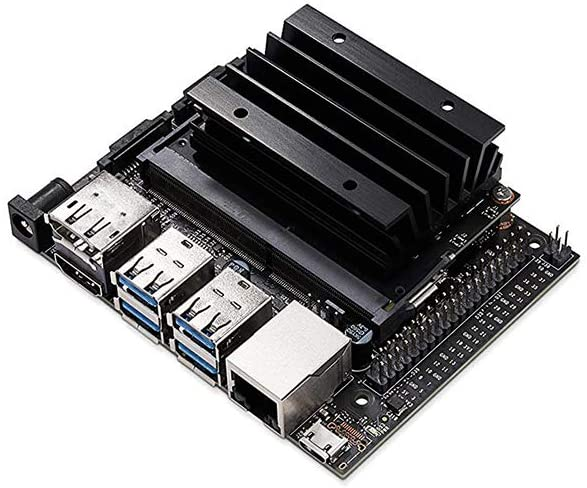
\includegraphics[width=.5\linewidth]{img/nanoboard}
  \captionof{figure}{NVIDIA Jetson Nano}
  \label{fig:nanoboard}
\end{minipage}%
\begin{minipage}{.5\textwidth}
  \centering
  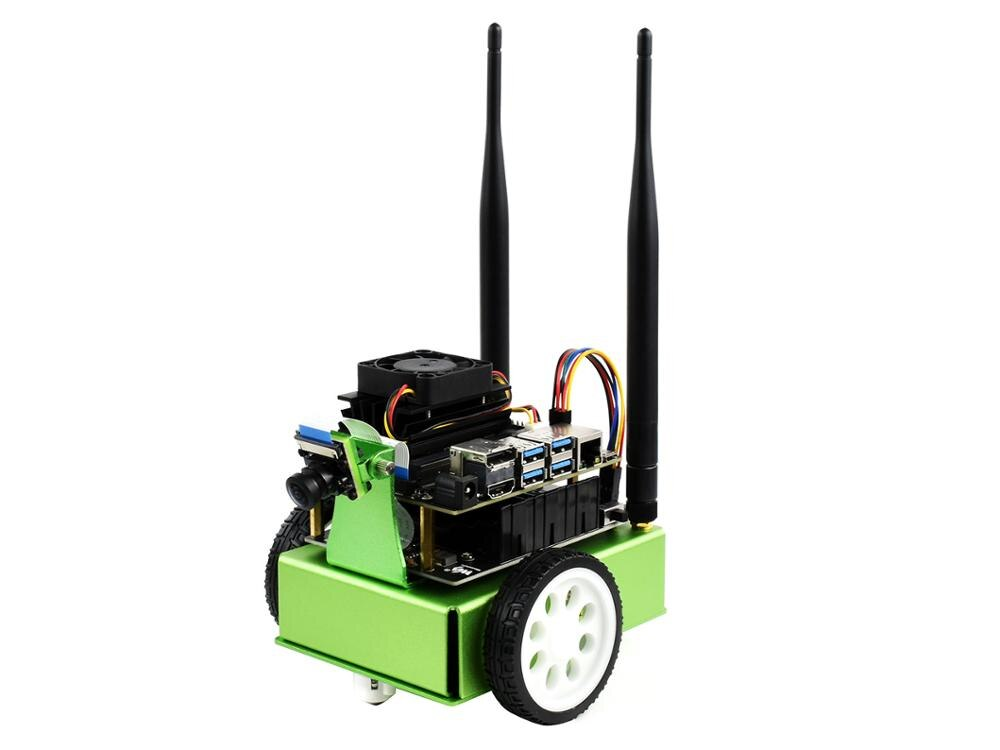
\includegraphics[width=.6\linewidth]{img/wavebot}
  \captionof{figure}{JetBot kit de Waveshare}
  \label{fig:wavebot}
\end{minipage}
\end{figure}

Hay variedad de opciones disponibles en el mercado, con kits robóticos que incluyen todo el hardware necesario para ensamblar un robot a partir de las piezas disponibles en el kit, así como la posibilidad de imprimir tus propios componentes y construir un robot desde cero utilizando una impresora 3D para ello. En este caso, se ha optado por utilizar un kit de calidad, que incluya todas las piezas, sensores y actuadores necesarios, además de hardware auxiliar, para facilitar la tarea y ahorrar tiempo en ensayo/error de diseño y ensamblaje. El kit escogido ha sido el proporcionado por la empresa Waveshare, que se puede ver en la Figura \ref{fig:waveboard}. Esta empresa es una tienda de componentes electrónicos, servicios y soluciones. Entre sus productos se encuentra el kit robótico denominado \textit{JetBot AI Kit}\footnote{https://www.waveshare.com/jetbot-ai-kit.htm} que incluye todas las piezas necesarias para la construcción de un robot pequeño, perfecto para el propósito de este proyecto. 

Se ha escogido este modelo en concreto por que está diseñado para montar una placa Jetson Nano (es el kit recomendado por NVIDIA), que es la que se ha elegido para este proyecto, además de por su calidad de materiales. El chasis está fabricado en una aleación de alumnio con acabado cepillado, incluye llantas de plástico prensado y neumáticos de goma con dibujo para un mejor agarre. Además el kit incluye un controlador para los motores, con \textit{sockets} para baterías que hace que el cableado sea trivial, no teniendo que lidiar con PCBs ni cables sueltos. Además, ofrece una cámara con un soporte en ángulo, un módulo wi-fi con dos antenas, un par de motores, ventilación, un joystick inalámbrico para la teleoperación, y herramientas para llevar a cabo el ensamblado del robot. Como único punto negativo, cabe destacar que la calidad de los motores no es la mejor, ya que carecen de par suficiente para un ajuste fino en velocidades bajas.

A continuación se detallan los componentes principales que componen este kit.

\subsubsection{Cámara}

El sensor que incluye la cámara de este kit es un IMX219-160. Este sensor es muy similar en características al de la cámara de la RaspberryPi (la PiCam). La Tabla \ref{tab:camera} condensa las especificaciones técnicas de esta cámara.

\begin{table}[H]
\centering
\captionsetup[table]{name=New Table Name}

\begin{tabular}{l|l} \hline
\textbf{Tamaño} & 25 mm (W) x 24 mm (L) \\ \hline
\textbf{Sensor} & Sony IMX219 \\ \hline
\textbf{Resolución} & 3280 (H) x 2464 (V) \\ \hline
\textbf{FOV} & 160º \\ \hline
\textbf{Distancia focal} & 3.15 mm\\ \hline
\textbf{Apertura} & 2.35\\ \hline
\end{tabular}
\caption{Especificaciones de la cámara}
\label{tab:camera}
\end{table}

Como se observa en la Tabla \ref{tab:camera} esta cámara dispone de una resolución de 3280x2464 píxeles (8 megapíxeles) con un FOV (\textit{Field of view}) de 160º debido a su gran angular. Puede trabajar a alta tasa de imágenes por segundo en función de la resolución a la que se trabaje, en concreto: 3280 x 2464 a 21 fps, 3280 x 1848 a 28 fps, 1920 x 1080 a 30 fps, 1280 x 720 a 60 fps, 1280 x 720 a 60 fps.


\subsubsection{Motores}

\textcolor{blue}{No sé si meter esta sección, los motores son genéricos} $\hookleftarrow$

El kit cuenta con un par de motores como actuadores principales del robot. En este caso concreto, estos motores DC son genéricos y no de demasiada calidad. Estos motores han sido una fuente de problemas durante todo el desarrollo del proyecto, ya que su falta de par, ha hecho casi imposible un control fino del robot a bajas velocidades.

\subsubsection{Placa controladora}

Este componente, que se puede observar en la Figura \ref{fig:waveboard} es el núcleo de este kit, ya que incorpora varios chips que ofrecen diferente funcionalidad, además de eliminar el trabajo de cableado casi al completo. La placa puede ser alimentada de dos formas: mediante baterías del tipo 18650 o mediante un adaptador de corriente de 12V. El zócalo de las baterías permite la carga de las mismas mientras la placa esté conectada a la corriente. Esta placa alimenta también a la Jetson Nano, mediante un regulador de voltaje APW7313, que porvee a la Jetson de 5V estables para su funcionamiento.

\begin{figure}
  \centering
  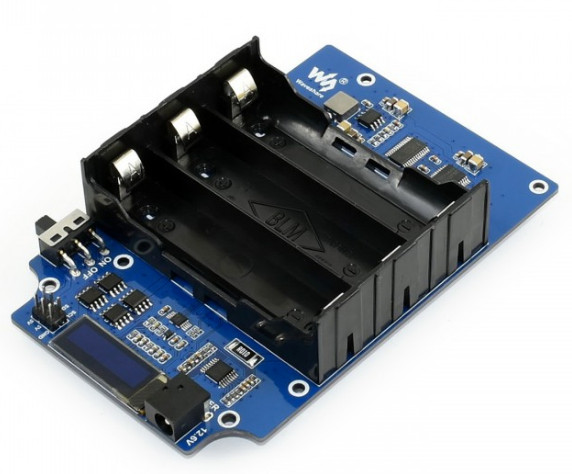
\includegraphics[width=.5\linewidth]{img/waveshare_board}
  \caption{Placa controladora del JetBot}
  \label{fig:waveboard}
\end{figure}

La función principal de esta placa es la de controlar los motores del robot, a través del protocolo I2C. Cuenta con conectores del tipo JST para ambos motores, que van directamente conectados a la placa. El chip controlador es un TB6612FNG dual H-bridge diseñado para trabajar con pequeños motores DC. El rango de voltajes soportado por este chip oscila entre los 4.5V y los 13.5V.

La placa cuenta además con una pantalla OLED de 0.91 pulgadas de una resolución de 128x32 píxeles, que muestra información sobre el robot como la dirección IP del robot, memoria RAM, tiempo de vida de batería, energía, etc. Esta pequeña pantalla resulta muy útil para comprobar de forma rápida el estado del robot sin necesidad de acceder a una terminal dentro del mismo. Para monitorear la batería en tiempo real, se utiliza el chip ADS1115 AD.

\subsubsection{Módulo Wi-Fi}

Otro componente principal de este kit es el módulo Wi-Fi, en este caso un módulo Intel AC-8265 de doble banda: 2.5 GHz y 5 GHz. En la Tabla \ref{tab:wifi} se resumen las especificaciones.

\begin{table}[H]
\centering
\captionsetup[table]{name=New Table Name}

\begin{tabular}{l|l} \hline
\textbf{Bandas} & 2.4 GHz, 5 GHz \\ \hline
\textbf{Velocidad máxima} & 867 Mbps \\ \hline
\textbf{Certificado} & 802.11 ac \\ \hline
\textbf{Bluetooth} & Sí \\ \hline
\end{tabular}
\caption{Especificaciones del módulo Wi-Fi}
\label{tab:wifi}
\end{table}

La inclusión de bluetooth del módulo lo hace especialmente útil para conectar periféricos como teclados, ratones o incluso joysticks para la teleoperación del robot. Adicionalmente, el kit de Waveshare cuenta con 2 antenas para ampliar el alcance de la señal, útil en exteriores o en entornos muy grandes donde el robot pueda estar alejado del computador.

\subsubsection{Joystick}

Como último aporte, este kit cuenta con un joystick inalámbrico para poder teleoperar el robot. Dado que el módulo inalámbrico que incluye el kit, soporta conexiones bluetooth, el joystick se puede conectar al mismo mediante un \textit{dongle} que viene incluído. Esta herramienta ha resultado útil en los primeros compases del proyecto para probar la mobilidad del robot, de forma sencilla. En la Figura \ref{fig:joystick} se puede ver este joystick.

\subsubsection{Pistas de Lego}

Como último elemento de este proyecto, se han utilizado pistas de Lego que han hecho las veces de circuito sobre el que el robot debía navegar. Debido al carácter modular de Lego, el intercambiar la forma de las pistas es tarea trivial. Es por ello que se decidió utilizar este elemento como pista para poder probar la solución del proyecto en diferentes formatos de circuito. La Figura \ref{fig:legos} muestra los módulos de Lego.

\begin{figure}
\centering
\begin{minipage}{.5\textwidth}
  \centering
  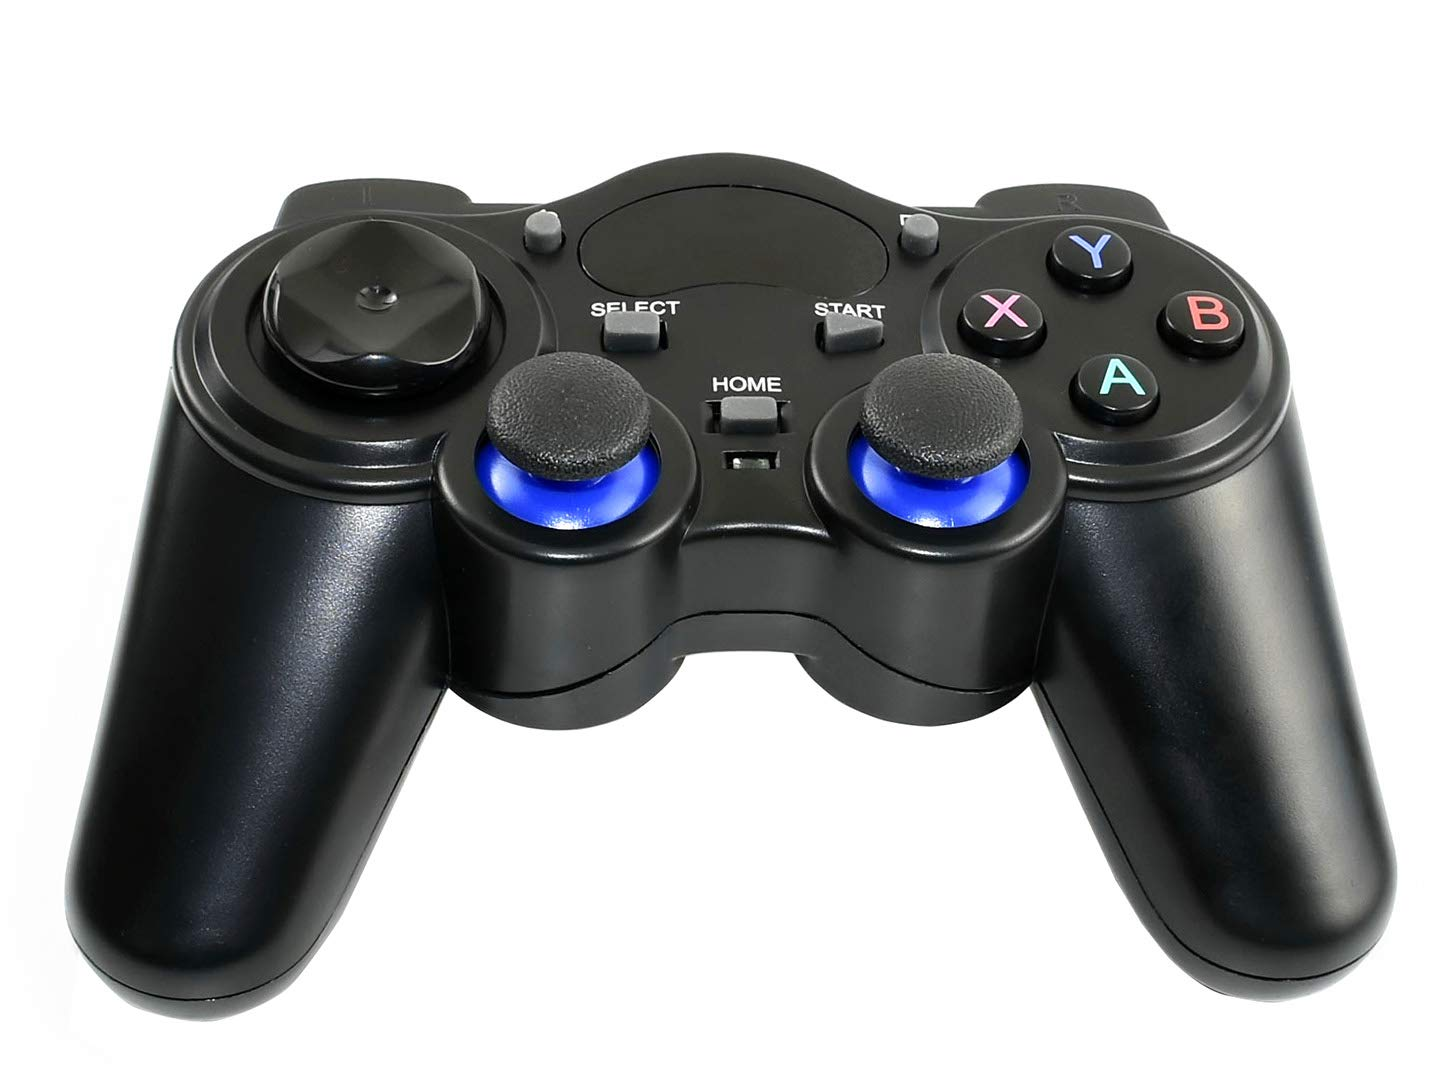
\includegraphics[width=.4\linewidth]{img/joystick}
  \captionof{figure}{Joystick de JetBot}
  \label{fig:joystick}
\end{minipage}%
\begin{minipage}{.5\textwidth}
  \centering
  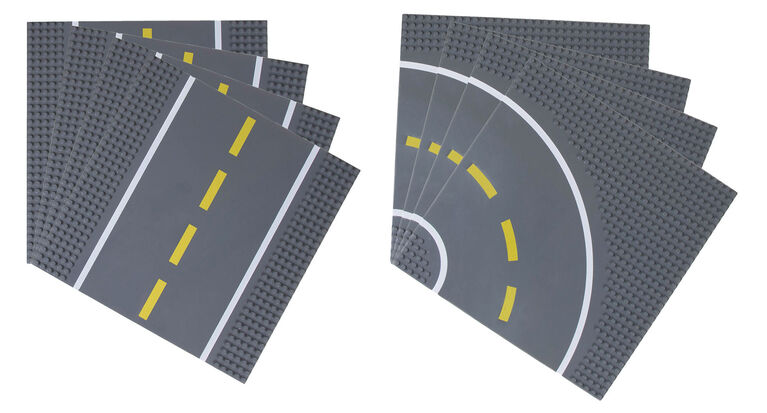
\includegraphics[width=.6\linewidth]{img/legos}
  \captionof{figure}{Módulos de lego}
  \label{fig:legos}
\end{minipage}
\end{figure}


\section{\textit{Software}}

En esta sección se enumeran y explican superficialmente todas las herramientas \textit{software} de las que se ha hecho uso durante el desarrollo del proyecto. Cada subsección describirá brevemente el componente en cuestión y el uso que se le ha dado en el proyecto. Se ha utilizado exclusivamente \textit{software} de código abierto.

\subsection{NVIDIA JetPack}
\label{sec:jetpack}

NVIDIA ofrece una gama de placas de alto rendimiento para sistemas empotrados, debido tanto a los avances en IA como en la necesidad cada vez más creciente de minimizar el tamaño de los computadores en diversos terrenos como, por ejemplo, el de la conducción autónoma. La NVIDIA Jetson Nano\footnote{https://developer.nvidia.com/embedded/learn/get-started-jetson-nano-devkit} es una de estas placas ya que está diseñada para trabajar como un computador de alto rendimiento en sistemas empotrados. En la sección \ref{sec:jnano}, se explica con relativo detalle las características de esta placa. Toda la gama, Jetson Nano, TX1, TX2, Xavier series, etc, siguen unas pautas de diseño muy optimizadas. La Jetson Nano en concreto implementa una versión adaptada de Ubuntu Linux, llamada NVIDIA JetPack que es desarrollada y mantenida por NVIDIA, y está disponible para ser descargada e instalada como el \textit{firmware} de la placa. Para el sistema desarrollado, la versión utilizada es JetPack 4.3; más precisamente, la imagen utilizada es una rama del JetPack 4.3 optimizada para el robot Jetbot (con la placa Jetson Nano). Esta implementación incluye interfaces de bajo nivel para implementar operaciones de computación en paralelo (usando CUDA), y varios SDKs de optimización (kits de desarrollo de software), como TensorRT, junto con interfaces para operar con los sensores y actuadores del robot. Además, contiene toda la infraestructura necesaria a nivel de software como CUDA, Pytorch, Python, etc. que mejor compatibilidad tienen con la versión de JetPack que se utilice. Este motor es de especial interés para este desarrollo, ya que permite aumentar enormemente la velocidad de inferencia sin perder precisión, gracias a sus optimizaciones.

NVIDIA JetPack se ha usado como SO (sistema operativo) base para la placa controladora Nano. Haber utilizado una distribución de Ubuntu (aunque fuera liviana) habría acarreado problemas de gestión de recursos como la CPU o la memoria a la hora de hacer inferencia en tiempo real, como se ha comprobado en la práctica.

\subsection{ROS}

Este proyecto se desarrolla haciendo uso del \textit{middleware} ROS (\textit{Robot Operating System}). Dada la necesidad de comunicación entre el robot y la plataforma BehaviorStudio, esta herramienta facilita la interconexión entre el \textit{hardware} y el \textit{software}.
ROS\footnote{https://www.ros.org} es un sistema meta-operativo de código abierto, que está mantenido por la \textit{Open Source Robotics Foundation} (OSRF). Al ser de código abierto, la comunidad ha desarrollado multitud de herramientas para ROS, que se integran y sincronizan continuamente con las versiones nuevas que lanzan. ROS proporciona un entorno distribuido compuesto por nodos, que son programas que se ejecutan de forma independiente tanto en local como en distribuido para realizar tareas individuales. Estos nodos se comunican de dos formas distintas: modo cliente-servidor entre nodos (modo síncrono) o meidante los denominados \textit{topics} (modo asíncrono). Los \textit{topics} de ROS se basan en comunicación estándar TCP/UDP mediante \textit{sockets}, y están ideados para comunicaciones unidireccionales y en \textit{streaming}, donde cada nodo puede ser publicador o subscriptor. En modo publicador, el nodo está escribiendo datos en un \textit{topic} determinado que un subscriptor estará comsumiendo. En modo subscriptor, el nodo estará consumiendo datos de un \textit{topic} que estará siendo actualizado por un publicador. Los datos que se leen/escriben en cada \textit{topic} siguen un determinado formato a través de mensajes de diversos tipos, según el propósito de la comunicación: mensajes de geometría, velocidad, posición, etc.

Una característica interesante de ROS es que ofrece un sistema de almacenamiento de \textit{topics} llamado ROSBags. Los ROSBags almacenan toda la información de los mensajes emitidos en el momento de la grabación en un solo archivo. Este archivo puede ser posteriormente reproducido para recuperar los mensajes de los \textit{topics} generados durante la grabación en el mismo orden en que fueron emitidos. Esto resulta útil especialmente para la grabación de conjuntos de datos, como imágenes de cámara, comandos de velocidad, de posición, etc., permitiendo al usuario realizar pruebas sobre el mismo conjunto de datos con diferentes modelos.

La versión de ROS utilizada para el desarrollo de este proyecto fue la \textit{tMelodic Morenia}, que era la LTS cuando el proyecto comenzó. Sin embargo, se está migrando a ROS \textit{Noetic Ninjemys} dado que es la actual LTS.

\subsection{Python}

Este trabajo ha sido desarrollado usando el lenguaje de programación Python\footnote{https://www.python.org}. Debido a algunos problemas de compatibilidad con la versión \textit{Melodic Morenia} de ROS 1, se ha optado por la utilización de la versión Python 2.7, aunque ha llegado a su fin de la vida útil. Esto se debe a que la implementación de ROS \textit{Melodic} está basada en Python 2.7 y no es compatible con algunas versiones más recientes de Python sin algunos ajustes previos. Sin embargo, BehaviorStudio es totalmente compatible con las nuevas versiones de Python (Python 3.6+) y la última versión de ROS1: ROS \textit{Noetic Ninjemys}, debido a que es agnóstico a la plataforma utilizada. 

Python se ha utilizado en este proyecto para el desarrollo íntegro de BehaviorStudio, así como todo el código auxiliar de entrenamiento del modelo y preprocesamiento de los datos.

\subsection{Pytorch}

Pytorch\footnote{https://pytorch.org} es una librería de cómputo numérico de alto rendimiento centrada en el cálculo en paralelo utilizando tensores como estructuras de datos estrella. Pytorch es una librería creada por la comunidad, de nacimiento reciente, en la que su principal ventaja frente a otros marcos como Tensorflow o Caffe es que utiliza grafos dinámicos en lugar de estáticos, mediante una técnica, que ellos denominan \textit{reverse-mode auto-differentiation}, que les permite cambiar el comportamiento de las redes neuronales de forma arbitraria sin coste adicional. Otra característica que hace muy potente a esta librería, es que está preparada de forma nativa para trabajar con GPU (\textit{Graphic Processing Unit} o con CPU (\textit{Central Processing Unit}) a placer, permitiendo además el cálculo distribuido de manera sencilla a través de métodos del API de la librería.

Pytorch tiene integración total con Python, lo que permite utilizar librerías de ciencias de datos como Numpy, Scipy, Scikit-learn, etc fácilmente. Un tensor en Pytorch es conceptualmente idéntico a uno de Numpy, lo que hace que ambas librerías se integren de forma nativa pudiendo aprovechar la potencia conjunta de las mismas, a la vez que simplifica la codificación de soluciones basadas en aprendizaje automático.

Debido a su gran simplicidad, la curva de entrada sencilla y la extensa documentación repleta de ejemplos de diversa índole, además de la integración con las placas Jetson de NVIDIA, se ha elegido este marco de trabajo como el principal para trabajar con las redes neuronales que se han desarrollado en este proyecto.

\subsection{OpenCV}

Para el procesamiento de imágenes en general, OpenCV\footnote{https://opencv.org} (\textit{Open Source Computer Vision}) es una biblioteca multilenguaje (Python, Java, C++) de código abierto (escrita nativamente en C++) para propósitos de Visión por Computadora. Entre los métodos clásicos que reúne, se pueden encontrar varias funciones adecuadas para el reconocimiento facial, la costura de imágenes, el seguimiento de los ojos, el filtrado de colores, etc.

Esta librería ofrece gran cantidad de algoritmos para manejar estructuras de datos, realizar modificaciones sobre las imágenes, detección de formas, etc. Debido a su gran eficiencia dada su integración con librerías de procesamiento de gráficos con GPU (NVIDIA CUDA y OpenGL), se ha convertido en la librería de visión artificial más usada por la comunidad tanto científica como por empresas; es decir, es el estándar \textit{de facto} en cuanto a librerías de procesameinto de imágenes.

Esta librería se ha utilizado como librería auxiliar y para realizar diferentes pruebas, como, por ejemplo, la implementación de una solución no basada en el aprendizaje a máquina para el robot simulado. Se ha utilizado la versión 4.4 de la biblioteca.

\subsection{Numpy}

La librería más potente para cálculo numérico y manejo de estructuras de datos complejas como los tensores es Numpy\footnote{https://numpy.org} (Numeric python). Esta librería, está diseñada para trabajar con Python, aunque está desarrollada en C++ para optimizar la eficiencia de la librería. Al igual que ocurre con OpenCV para el procesamiento de imágenes, Numpy se ha convertido en el estándar \textit{de facto} para el cálculo numérico. Con la irrupción de las redes neuronales, dado que estas trabajan principalmente con tensores, se ha popularizado aún más el uso de esta librería. El punto fuerte de esta librería es la optimización de todas sus operaciones, haciendo que las implementaciones manuales de la mayoría de ellas sea altamente ineficiente en comparación.

Todas estas capacidades hacen que Numpy sea una librería excelente para el manejo de estructuras de datos a bajo nivel, permitiendo operar sobre dichas estructuras de forma intuitiva y proporcionando métodos para facilitar las operaciones con ellas. A todo esto se suma que Numpy es un proyecto de código abierto, por lo que está en constante desarrollo y mejora gracias a la comunidad.

En este desarrollo, se ha utilizado Numpy como librería auxiliar para trabajar con los \textit{datasets} y con los tensores resultantes de las redes neuronales utilizadas.


\subsection{PyQt}

Qt es un conjunto de bibliotecas gráficas multiplataforma para desarrollar interfaces gráficas de usuario (GUIs). En nuestro proyecto se ha hecho uso de la librería Qt5 en su implementación en Python, que es la más estable hasta el momento. Debido a su carácter multiplataforma y multilenguaje, Qt dispone de diferentes APIs (\textit{Application Programming Interfaces}) en función del lenguaje de desarrollo que se utilice. Así por ejemplo disponemos de la versión para C++ denominada Qt, la versión para Java denominada QTJambi o la versión para python llamada PyQt, entre otras. Dispone tanto de versión gratuita como versión de pago destinada a soluciones empresariales.

Como la mayoría de bibliotecas gráficas, Qt ofrece una gran cantidad de elmentods de interfaz tales como: botones, scrolls verticales y laterales, cuadros de texto, separadores y un largo etc. Adicionalmente, ofrece una interfaz de communicaciones entre elementos basada en eventos, lo que facilita el paso de información y/o de disparadores para los elementos dinámicos de la interfaz de usuario. Qt cuenta además con un motor de animaciones y una librería 3D que se integra perfectamente en el código regular de la librería.

Esta librería se ha utilizado para el desarrollo de la parte visual de BehaviorStudio. Toda la interfaz gráfica se ha codificado utilizando exclusivamente PyQt5 y PyQt3D, sin la ayuda de IDEs como QtCreator.

\subsection{Gazebo}

Gazebo \footnote{http://gazebosim.org} es un simulador 3D que ofrece un entorno para desarrollar y probar sistemas multirrobot de manera sencilla. Es capaz de simular de forma realista muchos tipos de sensores y actuadores, entre os que destacan cámaras, láseres, sónares, GPS, etc, todo ello gracias, también, al motor de físicas que utiliza: Bullet, y a OpenGL (\textit{Open Graphics Library}). Además da soporte a multitud de robots tanto predefinidos, como definidos por el usuario. Gazebo es un \textit{software} de código libre, ya que está licenciado bajo la licencia de Apache 2.0 \footnote{http://www.apache.org/licenses/LICENSE-2.0.html}

Gazebo sigue a la cabeza de los simuladores de facto en la comunidad robótica del \textit{software} libre debido a su completitud y precisión. En la actualidad ya hay simuladores dedicados a la robótica como el AirSim de Microsoft \footnote{https://github.com/microsoft/AirSim} o la plataforma ISAAC de NVIDIA \footnote{https://developer.nvidia.com/isaac-sim}; no obstante Gazebo tiene integración nativa con ROS por lo que se ha escogido este simulador para este proyecto.

El hecho de que sea un simulador multirrobot dota de una gran utilidad a Gazebo, ya que se pueden simular infinidad de situaciones en las que uno o varios robots interactúen y estudiar su comportamiento de forma segura y controlada. Además, Gazebo ofrece la capacidad de ejecutarse de forma distribuida, lo que supone una gran ventaja frente a los demás simuladores.

El simulador Gazebo se ha utilizado para probar la plataforma BehaviorStudio para robots simulados.


\subsection{Otras herramientas}

Adicionalmente a las mencionadas arriba, se han utilizado otras librerías de manera circustancial que se mencionan a continuación:

\begin{itemize}
    \item \textbf{Pandas}\footnote{https://pandas.pydata.org}. Es un paquete Python de código libre que proporciona estructuras de datos rápidas y flexibles diseñadas para hacer que el  análisis / manipulación de datos. Se ha utilizado en este proyecto para la manupulación de los \textit{datasets} con los que se han entrenado las redes neuronales utilizadas.
    \item \textbf{Matplotlib}\footnote{https://matplotlib.org}. Es una biblioteca de graficado en 2D de Python que produce figuras de calidad en una variedad de formatos impresos y entornos interactivos a través de plataformas. Se ha utilizado en este proyecto para obtener las gráficas resultantes del entrenamiento de las redes neuronales.
    \item \textbf{Npyscreen}\footnote{https://npyscreen.readthedocs.io/introduction.html}. Es una biblioteca de widgets de python y un marco de aplicación para programar aplicaciones de terminal o de consola. Está construida sobre ncurses, que es parte de la biblioteca estándar. Se ha utilizado en este proyecto para construir una interfaz de usuario basada en terminal. Se incluye en esta sección ya que la implementación de esa interfaz de usuario está en fase de prueba de concepto.
\end{itemize}


\begin{comment}


In the following sections, examples of a figure, an equation, a table, a chemical structure, a list, a listing and a to-do note are shown.

\section{Figure}
\begin{figure}[H]
\centering
\includegraphics[width=0.45\linewidth, trim=3cm 11cm 3cm 11cm]{figure/X.pdf}
\includegraphics[width=0.45\linewidth, trim=3cm 11cm 3cm 11cm]{figure/Y.pdf}
\caption{Surface and contour plots showing the two dimensional function $z(x,y)=\sin(x+y)\cos(2x)$.}
\end{figure}

\section{Equation}
\begin{equation}
f(t)=\left\{ \begin{array}{ll}
1,~~~~ & t< 1 \\
t^2 & t\geq 1
\end{array}\right.
\end{equation}

\section{Table}
\begin{table}[H]
\centering
\caption{Values of $f(t)$ for $t=0,1,\dots 5$.}
\begin{tabular}{l|llllll} \hline\hline
$t$ & 0 & 1 & 2 & 3 & 4 & 5 \\ \hline
$f(t)$ & 1 & 1 & 4 & 9 & 16 & 25 \\ \hline\hline
\end{tabular}
\end{table}

\section{Chemical structure}
\begin{center}
\chemfig{X*5(-E-T-A-L-)}
\end{center}

\section{List}
\begin{enumerate}
  \item The first item
  \begin{enumerate}
    \item Nested item 1
    \item Nested item 2
  \end{enumerate}
  \item The second item
  \item The third item 
  \item \dots
\end{enumerate}

\section{Source code listing}
%\lstset{language=Matlab}
\begin{lstlisting}[frame=single]
% Generate x- and y-nodes
x=linspace(0,1); y=linspace(0,1);

% Calculate z=f(x,y)
for i=1:length(x)
 for j=1:length(y)
  z(i,j)=x(i)+2*y(j);
 end
end
\end{lstlisting}

\section{To-do note}
The \texttt{todo} package enables to-do notes to be added in the page margin. This can be a very convenient way of making notes in the document during the process of writing. All notes can be hidden by using the option \emph{disable} when loading the package in the settings. \todo{Example of a to-do note.}

\end{comment}